\documentclass{report}
\usepackage[french,english]{babel}
\usepackage{geometry}
 \geometry{
 a4paper,
 total={150mm,245mm},
 left=30mm,
 top=25mm,
 }
\usepackage{hyperref}
\usepackage[nodayofweek,level]{datetime}
\usepackage[utf8]{inputenc}
\usepackage[T1]{fontenc}
\usepackage[toc,page]{appendix}
\usepackage{float}
\usepackage{import}
\usepackage{amsmath} 
\usepackage[]{graphics}
\usepackage{graphicx}
\usepackage{caption}
\usepackage{subcaption}
\usepackage[usenames, dvipsnames]{color}
\usepackage{lipsum}
\usepackage{fancyhdr}
\usepackage{pdfpages}

\graphicspath{ {images/} }

\begin{document}
\selectlanguage{english}
\pagenumbering{gobble}
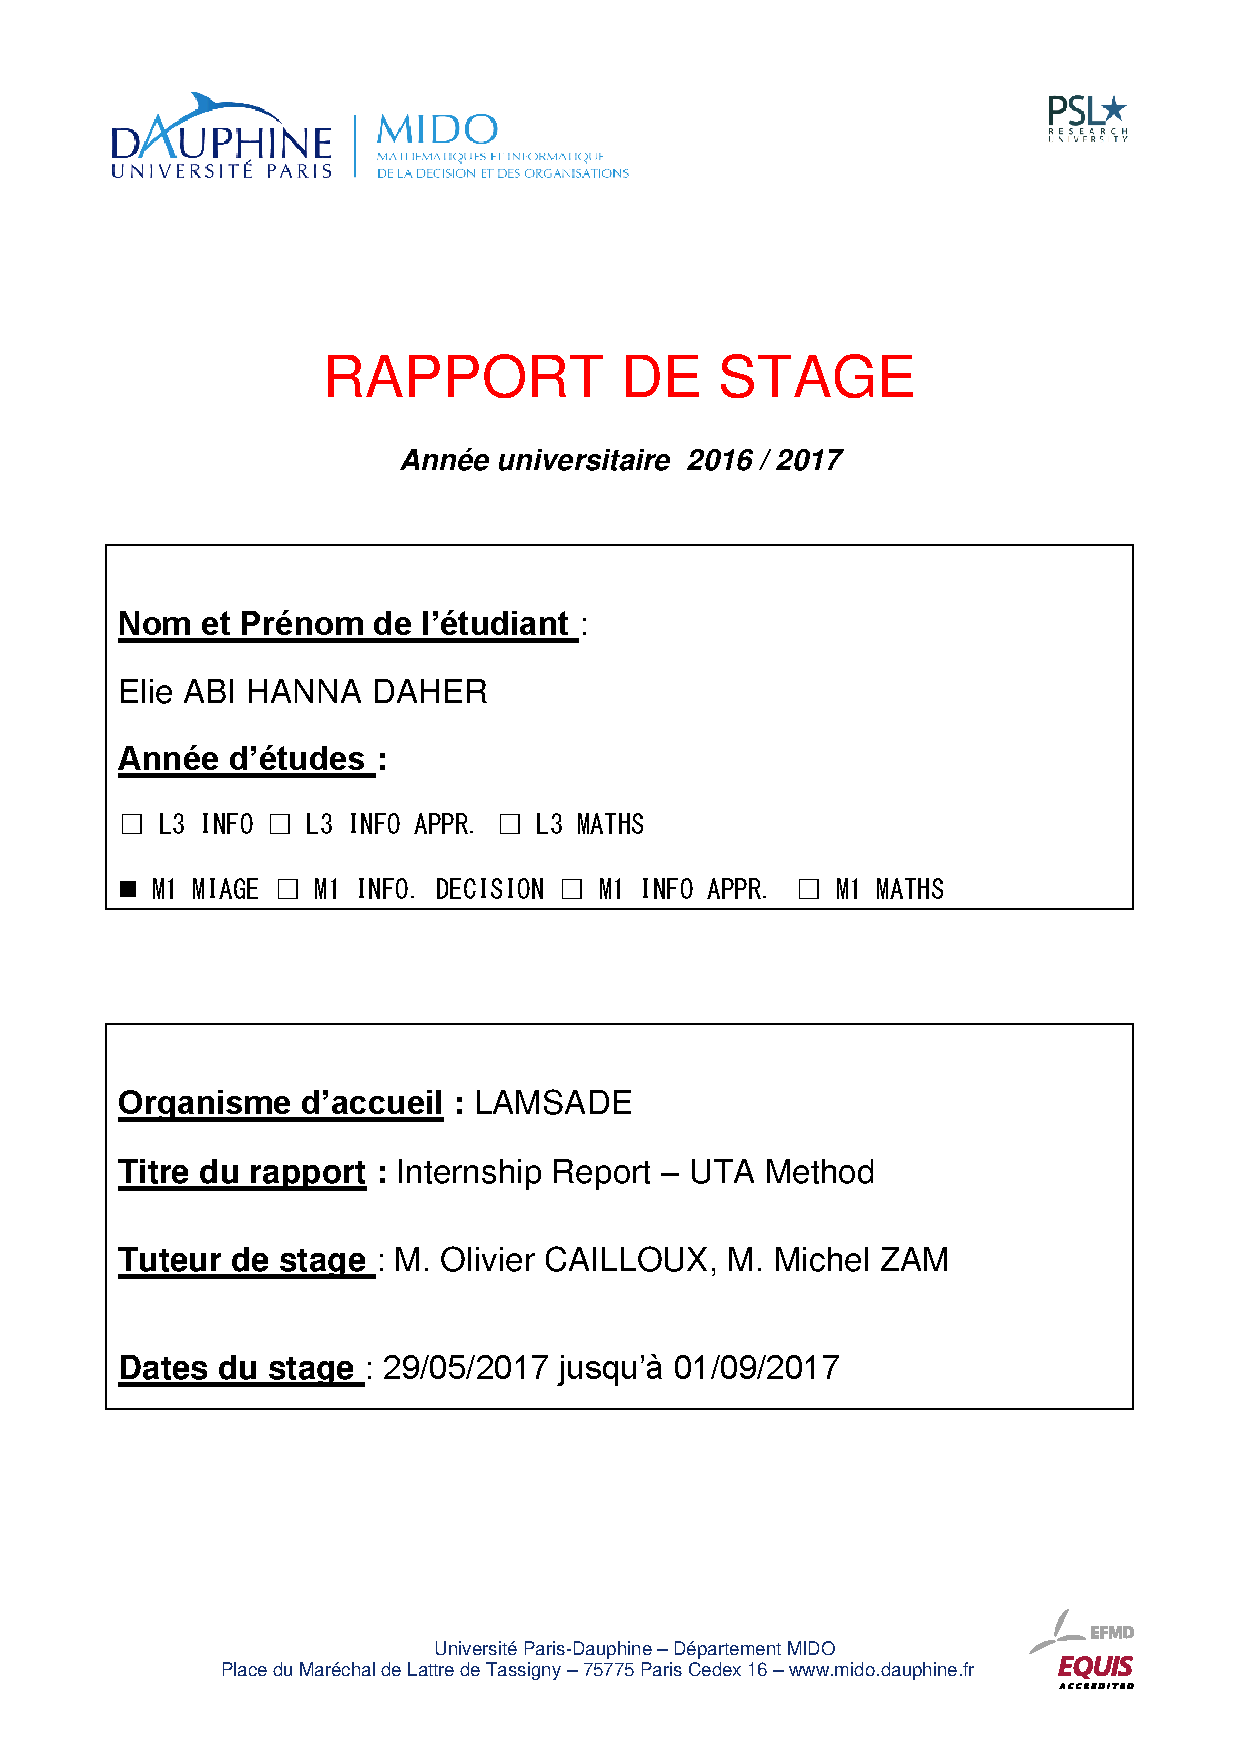
\includepdf{cover-page.pdf}

\abstract 
This report represents the work done during the internship at LAMSADE Dauphine, under the supervision of Mr. Olivier Cailloux and Mr. Michel Zam. The report gives an overview of the projects completed during this internship.\\
I have worked mainly on the UTA method, this procedure is an ordinal regression technique, proposed by E. Jacquete-Lagreze and J. Siskos, which adjust a system of additive utility function.

\newpage
{ \huge \bfseries Acknowledgment}\\[0.3cm]
\\

There is a few people that I would like to acknowledge for their help and contribution to the success of my internship at LAMSADE Dauphine.\\

First and foremost, I would like to thank Mr. Olivier Cailloux, a lecturer in computer science and researcher at LAMSADE. His advices and follow ups helped me a lot in completing my assignments during this internship.\\

I also would like to thank Mr. Michel Zam, the founder of KarmicSoft and an associate professor at Paris Dauphine University, for the opportunity given to me as an intern at LAMSADE\\

Doing my internship at LAMSADE with Mr. Cailloux and Mr. Zam was a pleasure, I have learned a lot from them , and I am grateful for this opportunity.\\

Finally I would like to thank the internship manager, Mrs Maude Manouvrier, for all her efforts in terms of follow-ups as well as her availability and patience to answer all my questions.\\

\newpage
\tableofcontents{}
\newpage
\pagenumbering{arabic}

\chapter{Introduction}
Currently I'm completing my master's degree in MIAGE at Paris Dauphine University so I had the opportunity to accomplish an internship at LAMSADE (Laboratoire d'analyse et modélisation de systèmes pour l'aide à la décision). LAMSADE is a Paris Dauphine research laboratory specialized in decision theoretic approaches. Decision theory aims to help individuals who face decision problems by elaborating a study of the reasoning and underlying agent's choices. \\

From \formatdate{29}{5}{2017} to \formatdate{1}{9}{2017}, I completed a research internship at LAMSADE. The internship was held under the supervision of Mr. Olivier Cailloux, a lecturer in computer science and researcher at LAMSADE and Mr. Michel Zam, the founder of KarmicSoft and an associate professor at Paris Dauphine University. I worked on my internship remotely, a weekly meeting was scheduled with Mr. Cailloux to get feedback on the work done. And I communicated with Mr. Zam via mails and calls. \\

This internship is very important for my professional career because it may be my last internship before I get my Master’s degree in Information systems for finance.  In addition, this internship allowed me to practice the different theoretical courses learned throughout my academic years.\\

One of the objectives of this fellowship is to propose the UTA method, that solves a multi-criteria problem by building a utility function based on the preferences of the Decision Maker, as an open source software component. Another objective is  to integrate this open source software into DecisionCloud, a software based on MyDraft which is a tool developed by KarmicSoft a LAMSADE spin-off. The research aspect represents an important objective in this internship. \\

In this internship report, I will describe the context of the project which contains an overview of the fellowship. While writing this report, I will describe the projects made: UTA, Linear Program Solver, UTA Calculator and the research realized. Finally I will conclude by reflecting on the flow of my internship. \\

\chapter{Context of the projects}
\section{Introduction to LAMSADE}
LAMSADE is a laboratory located in Paris Dauphine university. LAMSADE stands for Laboratoire d'analyse et modélisation de systèmes pour l'aide à la décision. The French laboratory has been established in 1974 by Bernard Roy. The main research subjects studied are operational research, decision aid, artificial intelligence (AI) and decision theory. \\
The activities of LAMSADE are divided into 3 poles: 
\begin{itemize}
\item Decision aid 
\item Combinatorial optimization and algorithmic
\item Data Science
\end{itemize}
LAMSADE is well known for the origin of the multiple-criteria decision analysis (MCDA), and for its approach of  the Algorithmic Decision Theory. The laboratory has established itself as the best research center internationally in it domain. \\
LAMSADE is structured in two  dimensions:
\begin{itemize}
\item Scientific 
\item Research
\end{itemize}
Scientific dimension represents the poles, where there is a community of researches invited to exchange throughout meetings and seminaries. The research dimension represents the projects assembled by the researches interested in the subject in question. Both of those dimensions are neither fixed neither permanent, they can be submitted to an evaluation by the Laboratory. 

\section{Objectives}
Throughout my  internship, I had several objectives to achieve and those objectives changed from when I began the internship. \\
The following list represents the objectives stated at the beginning of my fellowship: 
\begin{itemize}
\item Propose an open source software component of the UTA method (Main objective)
\item Integrate the UTA open software component as one of the tools in the Decision Deck community
\item Document, publish the software and implement a graphical user interface to the UTA by using DecisionCloud, a tool promoted by the Decision Deck
\end{itemize}

So as stated before, the objectives changed from the beginning of the internship for many reasons. We ended up doing an open source software component of the UTA method that we published on github instead of the DecisionCloud. This gave us the opportunity to evolve the software by doing more functionalities, and allowed us to grant more time for research. The main reason t we weren't able to make the tools in the Decision Deck community was because Mr. Zam wasn't available to assist me. So, we took this opportunity to make the software more developed.\\
During the internship the objectives were finally re-stated as follow: 
\begin{itemize}
\item Summarize UTA
\item Propose an open source software component of the UTA method
\item Generate Random alternatives and criteria
\item Generate Value Function
\item Search literature for existing similar studies, and how to generate realistic random alternatives
\end{itemize}

\section{Sharing of information}
All along the internship, all the work done was submitted on github so it can be seen by my supervisors. We held a meeting approximately each week, Mr. Cailloux and me, to discuss the conduct of the project and to get a feedback from him. Since I didn't have any colleagues to work with and only two supervisors, the communication was straight forward with my mentors. Only when I was having some serious difficulties that where complicating the work, I discussed with Mr. Cailloux via emails to solve it before the meeting. \\
Since Mr. Zam wasn't available during this summer at Paris, we shared some email and calls to talk about the progress of the internship. 

\section{Conduct of the internship}
On the \formatdate{29}{5}{2017} I started my internship. The first two weeks, were dedicated to get to know the platform MyDraft and create some basic applications. MyDraft is a platform created by KarmicSoft, and is  specialized in building and running data-driven Web applications. It is a platform for developing business applications the easiest way without complexity. During those two weeks, I did all the tutorials available on the site and in addition I created my own program. The project was called \textit{StockApp} where I recreated a project done during the course of \textit{Marché Financier}: Portfolio Management Project.\\

After learning about the platform MyDraft, I had my first meeting with Mr. Cailloux on the \formatdate{15}{6}{2017} where he introduced me a little bit to the UTA method and gave me the following book: \textit{Multiple Criteria Decision Analysis}, that contained a chapter explaining the UTA method. I had to understand this method and make a summary about it, so I took this opportunity to learn about LaTeX to create the summary. By the end of July, we created the summary of UTA method in Latex, and created my own problem to illustrate the method. Since one of the steps of the method was to solve a Linear Program,  we created an independent project to solve a simple Linear Program (LP) by using the google ortools (Optimization tools) library. Meanwhile, I made some research about literature for existing similar studies, and how to generate realistic random alternatives research. During this period, I had a weekly meeting with Mr. Cailloux.\\

By the end of the month of July, we had a meeting, Mr. Cailloux and me to discuss the software that will represent the UTA method. We designed the architecture, and I coded the program, it didn't take long because during the previous month I had already worked on little components of the software. For the month of august our goal was to finish this document, to make simulation and testing the software.\\ 

All of the work done is available as open source on my github repository: \url{ https://github.com/elieahd/decision-uta-method}.\\

Thus, in the next chapter, we will discuss the projects done above.

\chapter{Description of the projects}
\subsection{What is MyDraft}
MyDraft is a platform proposed by KarmicSoft. The goal of this platform is to develop a data and business driven application built only by click, without the need of a developer for a simple application. The application can be published in the Cloud and have a history of changes made on the data.\\

Another characteristic of MyDraft is the simplicity of coding which reduces the time required between creating the idea and accomplishing the app. MyDraft goal is to build a cloud-based agile development platform.\\

MyDraft proposes a unit testing and the possibility to generate UML model of the application. I couldn't test the last feature because of problems in the server located in United Kingdom.\\

\subsection{Projects - StockApp}
To practice using the platform MyDraft, I worked on my own application: StockApp. The project consists in collecting stock information and calculating the following information: 
\begin{itemize}
\item Weekly Returns of assets by calculating its mean and standard deviation. 
\item Correlation matrix of the stock returns
\item Correlation of stock returns with the stock market index
\item Beta, Sharpe Ratio and Treynor Ratio
\item Portfolio optimization scheme of Markowitz
\end{itemize}
I defined 3 classes in the model: 
\begin{itemize}
\item Stock
\item Data
\item Index
\end{itemize}
The class Stock has the following attributes: id, name, averageReturn, variance, standardDeviation, Beta, expectedReturn, sharpeRatio, growth, averageAdjClose\\
The class Data has the following attributes: returns, adjClose, date \\
The class Index has the following attributes: id, name\\
The stock has a relation 1 to many with Data, a stock has a list of Data. And the index has a relation 1 to many with Stock. \\
To achieve this project, I created an operation for the class Stock that calculates all the data needed.\\

In the IHM, I defined 3 tabs: list of index, list of stock and list of stock and Data.
\begin{figure}[H]
\centering
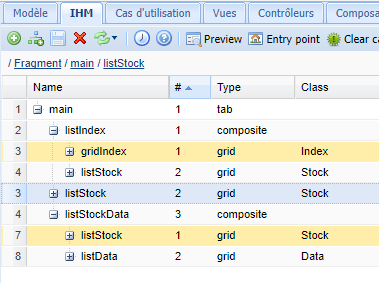
\includegraphics[width=10cm,height=5cm,keepaspectratio]{ihm.png}
\caption{MyDraft - IHM fragments}
\end{figure}

I succeeded in doing most of the functionalities of the project except for the last point, Portfolio optimization scheme of Markowitz, this wasn't possible to do in MyDraft since it needed the Macro used in the Excel.\\

\subsection{Tutorial}
On the Karmicsoft site, we can find a list of tutorials. The tutorials helped the users know how to use the platform. The following list represents all of the tutorials available on the site: 
\begin{itemize}
\item how to create an account on MyDraft 
\item how to define classes, objects and fragments
\item how to define state and operations
\item how to generate a use case diagram
\end{itemize}

All the before mentioned tutorials were made in French and published to YouTube. So, I took the initiative to create a PDF document in English on how to define classes, object and fragments. I thought that such tutorials would be interesting for non-speaking French and would be beneficial for MyDraft. The tutorials were sent to Mr. Zam.

\subsection{My remarks on MyDraft}
From my experience of using MyDraft, I found this platform very powerful and simple, on the other hand certain categories had some lacks or some bugs. Following is a list representing my remarks and where I think that MyDraft can be improved:
\begin{itemize}
\item MyDraft is not consistent with the language, we can find some words in English when the language chosen is French
\item not many tutorials are available in the tutorials section, and they are only in French
\item most buttons are not labeled, you only find an icon. So, figuring out what each button do is a bit confusing
\item there is no community nor documentation to help the users when they face a certain problem or bug
\item in certain scenarios, we may need to refresh the page so the changes can take place
\item generating UML model wasn't possible during my internship since there was a bug in the main server located in United Kingdom
\end{itemize}

But overall my experience with MyDraft was very good. This platform can have a real impact on the programming cycle which can lead to some new technology that can help the user create their own application without the need of a program thus speeding up the process.

\section{UTA}
\subsection{Introduction of the aid decision}
In decision theory, we elaborate a study of reasoning underlying the agent choices. Two branches can be deducted from the decision theory: giving an advice on how to make the best decisions and how existing agents make decisions. \\
In multiple-criteria decision analysis (MCDA), the following concepts play a fundamental role in decision-making problems: 
\begin{enumerate}
\item object of the decision, definition of the set of potential actions (alternatives) and the determination of a problem statement
\item modeling a consistent family of criteria
\item defining a global preference model
\item decision-aid or decision support
\end{enumerate}

\underline{Example: Buying a new car} \\
Let's consider we are trying to figure out which car to buy. Using the methodology presented above, we state that the objective of this problem is \textbf{buying a new car}. After stating the objective, we can now list the potential actions that represent the list of cars that we may buy. The potential action designates the object of the decision. An action is qualified as potential when it is deemed possible to implement or if it has some interest to the decision aiding process. So, the following list represent the potential actions for this example: 
\begin{itemize}
\item Peugeot 208 GTi
\item Nissan Sentra
\item Citroen C4
\item Peugeot 308 berline
\end{itemize}
After listing the list of potential cars, we can define a list of criteria that we will base our decision on. A criterion is constructed to evaluate and compare potential actions according to a point of view. When defining the list of criteria, you should always remember that they must be easy to evaluate (easy to convert to a scale) and should be logical.
Let's say we will base our purchase on the following criteria:
\begin{itemize}
\item price (in Euro)
\item comfort (0, +, ++, +++) \textit{0 being not comfortable and +++ very comfortable}
\item safety (1, 2, 3, 4, 5) \textit{1 being not safety and 5 safe}
\end{itemize}
During the decision process, we will determinate the global preferences of the potential actions:
\begin{enumerate}
\item Citroen C4
\item Peugeot 208 GTi
\item Peugeot 308 berline
\item Nissan Sentra
\end{enumerate}
Once the global preference is defined, we can start the decision support.\\

One of the multi-criteria decision analysis methods is the UTA method, which was proposed by E. Jacquet-Lagrèze and J. Siskos in 1982. This method is proposed by the Multi-Attribute Utility Theory (MAUT) that build a utility function based on the DM\footnote{Decision Maker} preferences.\\ 

The UTA method is used to solve a multi-criteria problem by building a utility function based on the preferences of the DM and solving a linear program (LP). It adopts the aggregation-disaggregation principles: where the model is based on a given preferences.\\ The UTASTAR, a variant of the UTA method, has been considered a better algorithm than UTA. Better result was found using the UTASTAR algorithm. So this is why we will focus on this method rather than the UTA method.\\The aim of the UTASTAR method is to estimate a set of additive utility functions which are as consistent as possible with the decision maker's preferences.\\
At the beginning of the problem, the DM should present the following information 
\begin{itemize}
\item rank of the actions
\item give the criteria he wants to base his decision on 
\item evaluate the action compared to the criterion
\end{itemize}
Once those information are presented, the UTASTAR algorithm can be executed. 

\newpage
\subsection{Principles and Notation}
Let's call $A={a,b,c,...}$ the set of potential actions and $g_1, g_2, g_3, ..., g_n$ the family of criteria. Where $g_i(a)$ represents the function of an action(alternative)$a$ on the criteria $g_i$ with $a \in A_R$. \\

We define $g_{i*}$ as the least preferred criteria: $g_{i*} = min_{a \in A} g_i (a)$ and $g_i^{*}$ as the most preferred criteria: $g_i^{*} = max_{a \in A} g_i (a)$. So the interval for each criteria $g_i$ is: $[g_{i*} , g_i^{*}]$.\\

If we want to evaluate two actions, for example $a$ and $b$, on only one criteria $g_i$ we have the following relations: 
\begin{equation}
\begin{cases}
a \succ b\Leftrightarrow g_i(a) > g_i(b) \quad preference\\
a\sim b \Leftrightarrow g_i(a) = g_i(b) \quad indifference \\
\end{cases}
\end{equation}
The criteria aggregation model in UTASTAR has the following form:
\begin{equation}\label{eq1}
v(g(a)) = \sum_{i=1}^{n} v_i (g_i (a))
\end{equation}
subject to normalization constraints:\\
\begin{equation}\label{eq2}
\begin{cases}
\sum_{i=1}^{n} v_i(g_{i}^{*}) = 1\\
v_i(g_{i*})= v_i(g_i^1) = 0, \forall i = 1, 2, ..., n\\
\end{cases}
\end{equation}
where $ v_i, i = 1,2,...,n$ are non-decreasing real valued function.\\
In UTASTAR we have 
\begin{equation}
w_{ij} = v_i(g_i^{j+1}) - v_i(g_i^{j}) \geq 0 \quad \forall i \quad j 
\end{equation}
Which will allow us to write: 
\begin{equation}
v_i(g_i^j) = \sum_{t=1}^{j-1} w_{it} \quad \forall i = 1,2,...,n \quad and \quad j = 2,3,...,\alpha _i -1 \\
\end{equation}
With the evaluation of an action a $g(a) = [g_1(a) , g_2(a) , ... , g_n(a)] $, we have the following relation:
\begin{equation}
\begin{cases}
v[g(a)] > v[g(b)] \Leftrightarrow a \succ b\\
v[g(a)] \sim v[g(b)] \Leftrightarrow a = b\\
\end{cases}
\end{equation}

\newpage
\subsection{Development} 
The updated version of UTA, UTASTAR, proposes a double error function for each action: $\sigma ^{+} (a)$ and $\sigma ^{-} (a)$. The value of each alternative $a \in A_R$ can be written: \\
\begin{equation}
v^{'} [g(a)] = \sum_{i=1}^{n} v_i [g_i (a)] - \sigma ^{+} (a)+ \sigma ^{-} (a) \quad \forall a \in A_R
\end{equation}
\begin{figure}[H]
\centering
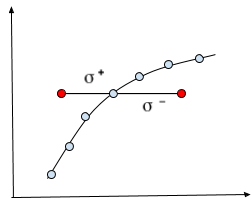
\includegraphics{error-function-utastar}
\caption{Error function in UTASTAR}
\end{figure}
For each criteria, the interval $[g_{i*}, g_i^{*}]$ is cut into $(\alpha _i -1)$ equal intervals, and the end points $g_i^{j}$ are given by the formula:
\begin{equation}
g_i^{j}= g_{i*} + \frac{j-1}{\alpha _i -1} (g_i^{*} - g_{i*}) \forall j = 1,2, ..., \alpha _i
\end{equation}
The marginal value of an action $a$ is calculated by a linear interpolation
\begin{equation}
v_i [g_i (a)] = v_i (g_i^{j}) + \frac{g_i (a) - g_i^{j}}{ g_i^{j+1} - g_i^{j}} [v_i (g_i^{j+1}) - v_i (g_i^{j}) ] 
\end{equation}
The set of reference actions $ A_R = a_1, a_2, ... , a_m$ is arranged by what $a_1$ is the best action and what $a_m$ is the worst action. Which indicate that we have two possible situations:
\begin{itemize}
\item $a_k \succ a_{k+1} \quad $ preference 
\item $a_k \sim a_{k+1} \quad $ indifference
\end{itemize} 
So if we have that $\Delta (a_k, a_{k+1} ) = v^{'} [g(a_k)] - v^{'} [g(a_{k+1})]$ and $\delta$ is a small positive number we will obtain the following relations: 
\begin{equation}\label{eq3}
\begin{cases}
\Delta (a_k, a_{k+1} ) \geq \delta\\
\Delta (a_k, a_{k+1} ) = 0 \\
\end{cases}
\end{equation}
The marginal value functions are estimated by means of the Linear Program with \eqref{eq1}, \eqref{eq2}, \eqref{eq3} as constraints, and an objective function depending on the $ \sigma^{+}$ and $\sigma^{-} $: 
$$ [min]z = \sum_{k=1}^{m} [ \sigma ^{+} (a_k) + \sigma ^{-} (a_k)] $$
subject to: 
\begin{equation}\label{eq5}
\begin{cases}
\Delta (a_k, a_{k+1} ) \geq \delta \quad or \quad \Delta (a_k, a_{k+1} ) = 0 \\
\sum_{i=1}^{n} \sum_{j=1}^{\alpha_i -1} w_{ij} = 1\\
w_{ij} \geq 0, \quad \sigma^{+}(a_k) \geq 0, \quad \sigma^{-}(a_k) \geq 0, \quad \forall i, j and k\\
\end{cases}
\end{equation}

\subsection{Example - Buying New Car}
The implementation of UTASTAR algorithm is illustrated by an example I made previously: \textbf{buying a new car}. Another example is available in the Appendices, Choice of transportation, taken from the book: Multiple Criteria Decision Analysis.\\ The DM is only interested in the following criteria:
\begin{itemize}
\item price (in Euro)
\item comfort ($0$, +, ++, +++) \textit{0 being not comfortable and +++ very comfortable}
\item safety ($1, 2, 3, 4, 5$) \textit{1 being not safety and 5 safe}
\end{itemize}
The evaluation of the previous criteria is presented in the following table: 
\begin{center}
\begin{tabular}{|c | c c c c|} 
\hline
Cars & Price & Comfort & Safety & Ranking of the DM \\ [0.5ex] 
\hline
Nissan Sentra (ns) & 17\,000 & +++ & 4 & 1 \\ 
\hline
Citroen C4 (c4) & 15\,000& ++ & 2 & 2\\ 
\hline
Peugeot 208 GT (p208) & 25\,000 & + & 3 & 3\\
\hline
Peugeot 308 berline (p308)& 18\,500 & 0 & 3 & 4\\
\hline
\end{tabular}
\end{center}
First of all, we should specify the scale \footnote{the interval $[g_{i*}, g_{i}^{*}]$ is cut into equal intervals} for each criteria.
\begin{itemize}
\item Price $\quad \Rightarrow \quad [g_{1*}, g_{1}^{*}] = [25\,000, 20\,000, 15\,000]$
\item Comfort $\quad \Rightarrow \quad [g_{2*}, g_{2}^{*}] = [0, +, ++, +++]$
\item Safety $\quad \Rightarrow \quad [g_{3*}, g_{3}^{*}] = [1, 3, 5]$
\end{itemize}
According to this formula: $v(g(a)) = \sum_{i=1}^{n} v_i (g_i (a))$ , the value of each alternative may be written: 
\begin{itemize}
\item $v(g(ns)) = 0.4v_1(15\,000) + 0.6v_1(20\,000) + v_2(+++) + 0.5v_3(3) + 0.5v_3(5) $
\item $v(g(c4)) = v_1(15\,000) + v_2(++) + 0.5 v_3(1) + 0.5v_3(3) = v_1(15\,000) + v_2(++) + 0.5v_3(3)$
\item $v(g(p208)) = v_1(25\,000) + v_2(+) + v_3(3) = v_2(+) + v_3(3) $
\item $v(g(p308)) = 0.3v_1(15\,000) + 0.7v_1(20\,000) + v_2(0) + v_3(3) = 0.3v_1(15\,000) + 0.7v_1(20\,000) + v_3(3)$
\end{itemize}
We have that $v_1(25\,000) = v_2(0) = v_3(1) = 0$. \\
Since the marginal value $v_i(g_i)$ can be expressed in terms of variables $w_{ij}$: $v_i(g_i^{j}) = \sum _{t=1}^{j-1} w_{it}$ , the value of each alternative can be written: 
\begin{itemize}
\item $v(g(ns)) = w_{11} + 0.4w_{12} + w_{21} + w_{22} + w_{23} + w_{31} + 0.5w_{32}$
\item $v(g(c4)) = w_{11} + w_{12} + w_{21} + w_{22} + 0.5w_{31}$
\item $v(g(p208)) = w_{21} + w_{31} $
\item $v(g(p308)) = w_{11} + 0.3w_{12} + w_{31}$
\end{itemize}
For each pair of consecutive alternatives, we express the difference between them: 
\begin{itemize}
\item $\Delta (ns,c4) = -0.6w_{12} + w_{23} + 0.5w_{31} + 0.5w_{32} -\sigma _{ns}^{+} +\sigma _{ns}^{-} +\sigma _{c4}^{+} - \sigma _{c4}^{-} $
\item $\Delta (c4, p208) = w_{11} + w_{12} + w_{22} - 0.5w_{31} -\sigma _{c4}^{+} +\sigma _{c4}^{-} +\sigma _{p208}^{+} - \sigma _{p208}^{-} $
\item $\Delta (p208, p308) =w_{21} - w_{11} - 0.3w_{12} -\sigma _{p208}^{+} +\sigma _{p208}^{-} +\sigma _{p308}^{+} - \sigma _{p308}^{-} $
\end{itemize}
Having $\delta = 0.05$, we can solve the following LP:\\

Objective: 
\begin{equation}
Minimize \quad \sum_{a \in A} \sigma _{a}^{+} + \sigma _{a}^{-}
\end{equation}

Subject to: \\
\begin{equation}
\begin{cases}
-0.6w_{12} + w_{23} + 0.5w_{31} + 0.5w_{32} -\sigma _{ns}^{+} +\sigma _{ns}^{-} +\sigma _{c4}^{+} - \sigma _{c4}^{-} \geq 0.05\\
w_{11} + w_{12} + w_{22} - 0.5w_{31} -\sigma _{c4}^{+} +\sigma _{c4}^{-} +\sigma _{p208}^{+} - \sigma _{p208}^{-} \geq 0.05 \\
w_{21} - w_{11} - 0.3w_{12} -\sigma _{p208}^{+} +\sigma _{p208}^{-} +\sigma _{p308}^{+} - \sigma _{p308}^{-} \geq 0.05 \\
w_{11} + w_{12} + w_{21} + w_{22} + w_{23} + w_{31} + w_{32} = 1
\end{cases}
\end{equation}
An optimal solution is $w_{12} = 0.34$, $w_{21} = 0.152$, $w_{32} = 0.51$ with $\sum_{a \in A} \sigma _{a}^{+} + \sigma _{a}^{-} = 0$. The utilities found for each alternative are as follows: \\ 
\begin{itemize}
\item $v(g(ns)) = 0.543$
\item $v(g(c4)) = 0.492$
\item $v(g(p208)) = 0.152 $
\item $v(g(p308)) = 0.102 $
\end{itemize}
Those utilities are consistent with the DM's preference ranking. \\

The UTA method build a utility function based on the preferences of the DM and consists in solving a linear program (LP) to resolve a multi-criteria problem.\\
This method will elaborate a model of preferences which is as similar as possible to the DM's preferences.\\
The improved version of the UTA, UTASTAR, has performed better than the regular method.

\subsection{Value Function}
The value function of a problem will allow you to calculate the value of each alternative.\\
It is composed of several partial value functions, each one represents a criterion with the intervals that represent the coordinates of several points.\\
So the following partial value function is of the criterion that have the following scale: $[1000,2000,3000]$
\begin{figure}[H]
\centering
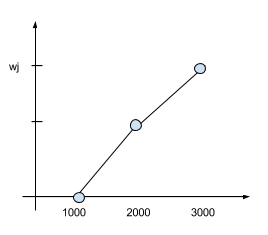
\includegraphics[width=10cm,height=5cm,keepaspectratio]{pvf.png}
\caption{UTA - Partial Value Function}
\end{figure}
So the sum $w_j$ of all the partial value functions represented in the upper figure is equal to 1.\\

\section{Linear Program Solver}
One of the steps of the UTA algorithm is solving a Linear Program. To complete the UTA algorithm, I created an independent java application that has the objective of solving the LP by finding the optimal solution.\\
To achieve this goal, I had to use the google ortools (Optimization tools) library. The library is composed of two external jar files: \textit{com.google.ortools.jar} and \textit{protobuf.jar} and of one native class library \textit{jniortools.dll}. You can find these libraries in the github repository under src/libs.
\begin{figure}[H]
\centering
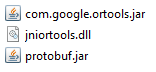
\includegraphics[width=4cm,height=1.5cm,keepaspectratio]{lp-libs.png}
\caption{Library used in the solver}
\end{figure}
Let's consider the following example:\\

Objective: 
\begin{equation}
Maximize \quad 10x_1 + 6x_2 + 4x_3
\end{equation}

subject to: \\
\begin{equation}
\begin{cases}
x_1 + x_2 + x_3 \leq 100\\
10x_1 + 4x_2 + 5x_3 \leq 600\\
2x_1 + 2x_2 + 6x_3 \leq 300\\
\end{cases}
\end{equation}
To solve the LP, we need to create an instance of the solver:
\begin{figure}[H]
\centering
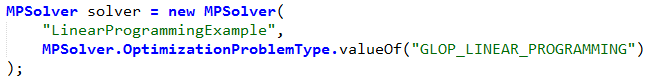
\includegraphics[width=\textwidth]{lp-solver.png}
\caption{Java code to define the solver}
\end{figure}
After that, we define the 3 variables $x_1$, $x_2$ et $x_3 \quad \in \quad [0 ; \infty]$: \\
\begin{figure}[H]
\centering
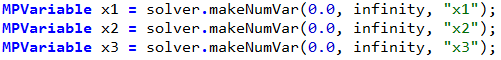
\includegraphics[width=10cm,height=3cm,keepaspectratio]{lp-variables.png}
\caption{Java code to define the variables of the LP}
\end{figure}
We define the objective $Maximize \quad 10x_1 + 6x_2 + 4x_3$: \\
\begin{figure}[H]
\centering
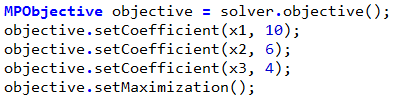
\includegraphics[width=8cm,height=2cm,keepaspectratio]{lp-objectif.png}
\caption{Java code to define the objective of LP}
\end{figure}
We do the same for the constraints: \\
\begin{figure}[H]
\centering
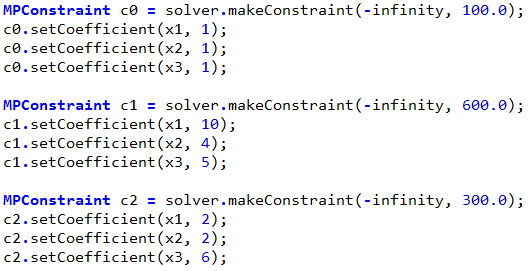
\includegraphics[width=10cm,height=6cm,keepaspectratio]{lp-constraints.png}
\caption{Java code to define the constraints of the LP}
\end{figure}
After setting all the constraints and variables we can execute the solver: \\
\begin{figure}[H]
\centering

\includegraphics[width=10cm,height=6cm,keepaspectratio]{lp-solve.png}
\caption{Java code for running the solver}
\end{figure}
After executing the solver, we display the optimal value of the objective and the value of the variables: \\
\begin{figure}[H]
\centering
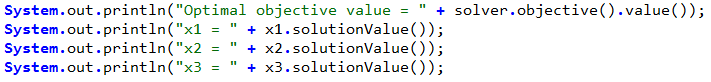
\includegraphics[width=\textwidth]{lp-result.png}
\caption{Java code for displaying the result of the solver}
\end{figure}
Once you run the program, you will have the following the result: 
\begin{center}
Optimal objective value = 733.3333333333\\
x1 = 33.33333333336\\
x2 = 66.66666666666\\
x3 = 0.0\\
\end{center}

\section{Research}
One of the most important aspect of this internship is the research. The objective of the research was to find similar studies, how to generate realistic random alternatives and studies made on UTA method.
\subsection{Comparative analysis of UTA multicriteria methods}
The paper Comparative analysis of UTA multicriteria methods, written by Michel Beuthe and Giuseppe Scannella, is mainly about the variants of UTA method. As discussed in this paper a method of multi-criteria analysis is chosen depending on the circumstances of the decision making. UTA makes the estimation of a nonlinear additive function possible, which is obtained using a linear program. The only information required from the decision maker is the global preferences between projects. \\
After the execution of the algorithm, it is possible to evaluate the preference stated by the decision maker.\\
Another point stated in the paper is that the initial value of $\delta$ must not be given too high. In the basic model, it was noted that the values given to $\delta$ were to some extent arbitrary. 
\subsubsection{Simulations}
The simulation is applied to the case of 353 road projects in Belgian Network during the period 1985-2010. The Center of Road Research (CRR) realized a multi criteria analysis that used 29 criteria regrouped in six main themes: 
\begin{itemize}
\item safety on the present road
\item projects socioeconomic aspects
\item impact on environment
\item current and future traffic
\item problems of planning and urbanism
\item wear state of the current road.
\end{itemize}
The 29 criteria have been sorted with a scale going from 1 to 5. 

\subsubsection{Variants of UTA}
\begin{enumerate}
\item UTA
\item UTASTAR
\item UTA2
\item UTAMKEN
\item UTAMP1
\item UTAMP2
\item UTAMIME
\item UTASTARMIME
\item UTA2MIME
\end{enumerate}

\subsubsection{Conclusions made}
When there is no error in the utility function estimation, $ \sum_{a \in A} \sigma _{a}^{+} + \sigma _{a}^{-} = 0$, the basic UTA method provides the most practical and efficient method of estimation. \\
Even when there is interdependence between criteria, the UTA approach provides good results. \\
In the case where the utility function estimation is positive, $ \sum_{a \in A} \sigma _{a}^{+} + \sigma _{a}^{-} >0 0$, the UTASTAR appears more reliable.\\
The simulations results indicate that small value of $\delta$ lead to better results in case of a positive utility function estimation. But in case of no error in the utility function estimation, larger value of $\delta$ can provide better results. The use of UTAMP1 or UTAMP2 may then be used to find the practical upper bound of the values given. 

\subsection{Disadvantages of the UTA method}
\begin{enumerate}
\item We can always question the decision marker about his preferences\\
The UTA method need the alternatives and action list given with their preferences. The preferences should be given by the DM, so if he made a mistake or a wrong estimation of the preference the linear program can have a wrong constraint which can affect the final results. 
\item Solution may not be the only one as in any LP we can have multiple solutions\\
A step of the UTA is solving a linear program and as we all know linear program can have different solutions each time we run the LP.
\end{enumerate}

\subsection{Experimentation about the variant of UTA, UTASTAR and UTA}
An experimentation was made by J. SISKOS and D. YANNACOPOULOUS and was written in the paper: \textit{Amélioration de la méthode UTA par introduction d'une double fonction d'erreur} which is the \textit{Cahier du LAMSADE n49}. The goal of this experimentation was to show the advantages offered by the newer version of UTA compared to the older version. Ten actions have been evaluated randomly over six criteria with a scale of $[1,4]$ where four is the most preferred value.\\

In order to facilitate the comparison, two factors have been used:
\begin{enumerate}
\item Iterations necessary to obtain the optimal utility
\item Objective of the LP: Minimization of $ \sum_{a \in A} \sigma _{a}^{+} + \sigma _{a}^{-} $ 
\end{enumerate}

The first factor was better by $48\%$ than the older version. The second factor was better by $36\%$ than the older version. 
Comparison table:

\begin{center}
\begin{tabular}{| c | c | c | c |} 
\hline
Factors & UTA & UTASTAR & Result \\
\hline
Iterations & $21.5$ & $11.1$ & drop of 48\% \\ 
\hline
Objective of LP & $0.34$ & $0.53$ & drop of 36\%\\ 
\hline
\end{tabular}
\end{center}

\newpage
\section{Implementation - UTA Calculator}
We wanted to implement the UTASTAR method. In order to make it possible, we created a java program: uta-calculator. Basically, our goal was to generate a decision problem and run the UTASTAR algorithm. \\
Another objective we were trying to achieve was to generate random alternatives and criteria, so we can generate a decision problem. \\
After running the algorithm, our goal was to get the $v^{R}$ and $v^{T}$ and compare them. 
\subsection{Architecture}
\subsubsection{Class Diagram}
\begin{figure}[H]
\centering
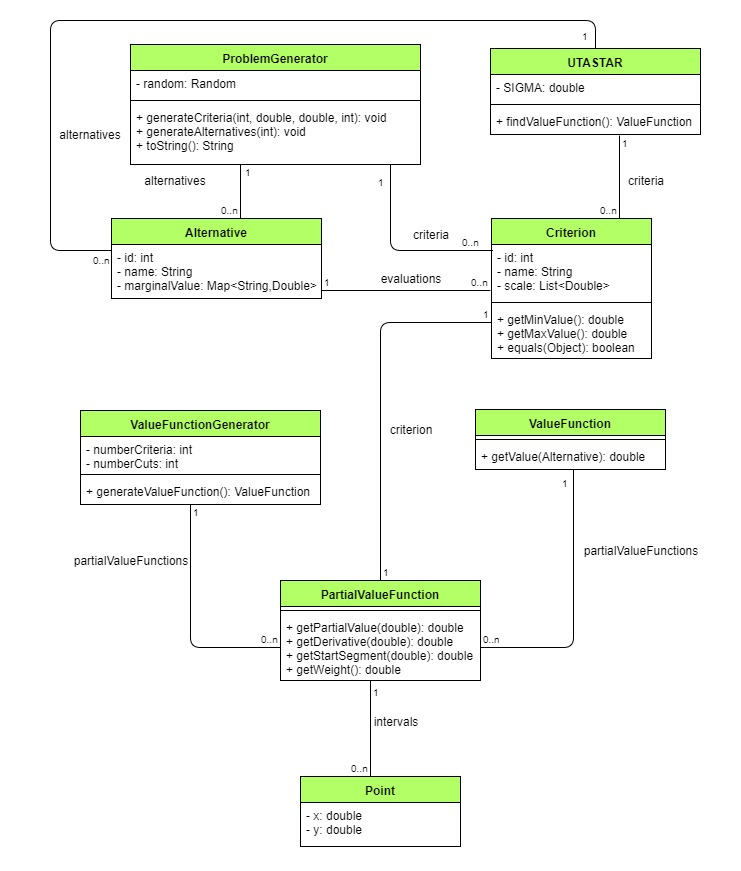
\includegraphics[width=17cm,height=17cm,keepaspectratio]{diagram-uml.png}
\caption{Class Diagram}
\end{figure}
Other than the external libraries used in the resolution of a LP, we used the library commons-math from Apache which helped us by calculating the average and standard deviation of the results obtained during the simulation. \\

\subsubsection{Maven}
Since we wanted to create an open source project, following the standards conventions was a must which led us to the use of Maven. \\

We figured out that we need to configure our project in Maven. Maven has been created to make a standard way to build a project and a way to share JAR files through many projects. Figuring out dependencies for small projects is not hard, but once the dependencies expand it will get out of hand. Another plus of using Maven is that it provides a quality project information.\\

I personally prefer using the IDE Eclipse Luna to code in Java and I am currently using the version Luna 4.4.2 . Using Maven  won't be a problem for people who don't use Eclipse, they can use NetBeans or IDEA or any other IDE that supports Maven. \\

\underline{Configuration of Maven: }
\begin{itemize}
\item groupId: io.github.oliviercailloux
\item artifactId: uta-calculator
\end{itemize}

\subsection{Functionalities}
The following list represents the functionalities of the program I worked on:
\begin{itemize}
\item Program your own decision problem
\item Generate a random decision problem
\item Solve the decision problem by using UTASTAR algorithm
\item Elaborate a ValueFunction from a decision problem
\item Generate a ValueFunction
\item Publishing the application as an open source
\end{itemize}
\subsection{Utils}
To make some functions more generic, we created a package called utils, where we can find two java classes: 
\begin{itemize}
\item NumbersGenerator
\item ScaleGenerator
\end{itemize}

\subsubsection{NumbersGenerator}
The goal of this util class is to generate decimal numbers that have a certain sum. For example, creating three numbers that have the sum of 1. \\
To make this possible, the class NumbersGenerator follows the method generate that takes the following as parameters: 
\begin{enumerate}
\item counter (int)
\item targetSum (double)
\end{enumerate} 
The parameter counter represents the counter of numbers we want to generate, and the parameter targetSum represents the sum we are targeting. \\
You can specify the Random value in case you want to have the same result when doing testing. \\
This method will return a List of number of type double. 

\subsubsection{ScaleGenerator}
The goal of this util class is to generate scale for a criterion, where the interval $[minValue, maxValue]$ is cut into equal intervals. For example, If you want the scale of a criterion that have 10 as minimum value, 20 as maximum value and with four cuts, the function should return the following list: $[10.0, 13.333, 16.667, 20.0]$.\\
To make this possible, the class ScaleGenerator follows the method generate that takes the following as parameters: 
\begin{enumerate}
\item minValue (double)
\item maxValue (double)
\item cuts (int)
\end{enumerate} 
The parameter minValue represents the minimum value of a criterion, the parameter maxValue represents the maximum value of a criterion and the parameter cuts represents the numbers of cuts into which you want to cut the interval. \\
This method will return a List of numbers of type double. 

\subsection{Inputs and outputs of the UTASTAR}
In order to generate a problem, you have two possibilities:
\begin{itemize}
\item Generate a random problem
\item Creating your own problem
\end{itemize}
To \textbf{generate a random problem}, you have to specify the following inputs when running the\textit{MainRandomProblem} java class.:
\begin{itemize}
\item criterion information
\begin{itemize}
\item numbers of criteria
\item minimum and maximum value of a criterion
\item number of cuts of the scale of a criterion
\end{itemize}
\item numbers of alternatives
\end{itemize}
By having the following inputs, the software will create the alternatives and criteria and run the UTASTAR algorithm.\\
To \textbf{create your own problem} all you have to do is create a list of criterions and a list of alternatives in the code java, and run the algorithm by giving them parameters. The example of \textbf{Buying New Car} is available in the \textit{MainBuyingNewCar} java class. \\

As output, both possibilities will display the results of the UTASTAR algorithm, value function and the value of each alternative.\\

\subsection{Simulation and Comparison}
In order to calculate the average and the standard deviation I used the external library: Commons Math: The Apache Commons Mathematics Library. This library is lightweight, easy-to-use and can do the statistics formula.

\subsection{Future Improvements}
This program has been done during my three months’ internship. It didn't take three months to make this program, but in order to make such a program I had to do a research and learn about the UTA method. Basically, we had to compromise on some functionalities in order to make the implementation easier. Since the program will be available as an open source on GitHub, it has the potential to grow with some improvements. The following list is some of the improvements that could be made:\\
\begin{enumerate}
\item in the current version of the program, the criterion evaluation has a minimum value and a maximum value, so the evaluation of an action is made in the range $[minValue, maxValue]$ with minValue being the least preferred criterion and maxValue the most preferred. But what if we want to represent a criterion that has maxValue as the least preferred criterion and minValue as the most preferred, like the criterion price, in the current version, this won't be possible. 
\item in our program, a criterion has a minimum value and a maximum value, but what if the criterion is not a quantitative item, not evaluated in numbers. For example, let's say we want to evaluate the comfort, we can have the following values: 0, +, ++, +++ or not comfortable, basic, comfortable, very comfortable. So as an improvement we can expect to be able to design all of the criterions possible. 
\item the current version doesn't support a graphical interface, a graphical interface can be handy to make the software more user friendly. 
\end{enumerate}

\section{Conclusion on the projects}
During the internship, a lot of tasks has been accomplished. First, I have been able to learn about the platform MyDraft, to make a tutorial and to realize a small application. Secondly, I was able to learn about a new decision method, UTA, where I made a summary about it, and created my own problem, Buying New Car. Before implementing the UTASTAR method, a research was made. The goal of the research was not fully achieved, its objective was to find similar studies made, how to generate realistic random alternatives and studies made on UTA method. I was able to find some literature about similar studies and the UTA method but I couldn't find how to generate realistic random alternatives and criteria since I didn't have a lot of time to search for it. And finally, I was able to implement the UTASTAR method and make a simulation to extract the results from it. \\

During the implementation, we used some external libraries that were given by Mr. Cailloux. The libraries provided by my supervisor were handy and very lightweight. We published the work done and the source code on Github, I believe that this was a great choice since we were aiming to provide an open source software and there is no better way than Github. The code was done in Java which helped us to find some external libraries.\\


\chapter{Conclusion}
\section{Difficulties encountered}
I didn't have many difficulties, the only main problem I faced was the fact that I was working alone. Working alone and not surrounded by colleagues can be a little set back, since you cannot interact with them and ask questions on the spot. I had to wait for the next meeting or send an email in case I had any inquiries or problems.\\

\section{Personal benefits}
During my internship at LAMSADE, I have learned a lot, put in practice many of the subjects learned during my academic years, so here the list of my new acquired skills: 
\begin{itemize}
\item Learning to write documents using LaTeX which helped with the appearance of documents to focus more on the content. 
\item Learning a new Decision method, the UTA method
\item Re-doing my project of Portfolio Management was helpful for me since next year I will be completing my master’s degree in Information System for finance
\item Learning how to make research of literature on a certain subject 
\item Making projects using Maven
\item Publishing a software on github as open source
\item Practicing my English skill\\
\end{itemize}

The internship has been very rewarding for me on several levels, being able to practice several subjects taken during my academic years like the course \textit{Decision}, \textit{Marché Financier} and \textit{Advanced Java}. Due to this internship, I learned how to be autonomous and how to learn to manage my own time to finish the work.\\
To sum-up, these three months internship were a great experience on a professional level and a personal level.

\begin{thebibliography}{9}
\addcontentsline{toc}{chapter}{Bibliography}
\bibitem{multiple-criteria-decision-analysis} GRECO S., EHRGOTT M., RUI FIGUEIRA J., 2004, \textit{Multiple Criteria Decision Analysis}
\bibitem{cahier-lamsade-24} SISKOS J., 1979, \textit{Cahier du LAMSADE n24 : Les programmes UTA}
\bibitem{cahier-lamsade-49} SISKOS J., YANNACOPOULOS D., 1982, \textit{Cahier du LAMSADE n49 : Amélioration de la méthode UTA par introduction d’une double fonction d’erreurs}
\bibitem{these-hammami} HAMMAMI A., 2003, \textit{Thèse : Modélisation technico-économique d’une chaîne logistique dans une entreprise reseau}
\bibitem{study-stock-ranking} LUO H., SUN Z., 2014, \textit{A study on Stock Ranking and Selection Strategy Based on UTA Method under the Condition of Inconsistence}
\bibitem{multicriteria-decision-aid-methodology} ZOPOUNIDIS C., DOUMPOS M., 1997, \textit{A multicriteria decision aid methodology for the assessment of country risk}
\bibitem{development-utastar-method-fuzzy} EHSANIFAR M., ESHLAGHI A., KERAMATI M., NAZEMI J., 2013, \textit{The Development of UTASTAR Method in Fuzzy Environment for Supplier Selection}
\bibitem{application-methode-uta} SISKOS J., 1983, \textit{Application de la méthode UTA à un problème de sélection de points de vente mettant en jeu des critères multiples}
\end{thebibliography}

\listoffigures
\addcontentsline{toc}{chapter}{Table of figures}

\begin{appendices}

\selectlanguage{french}
\chapter{Compte Rendus avec M. Cailloux}
\section{CR1 - 15 juin 2017}
\textbf{15 juin 2017} / 15:00 / Université Paris Dauphine \\

\underline{Participants} \\

Olivier Cailloux, Elie Daher\\

\underline{Déroulement de la réunion}\\
\begin{itemize}
	\item Explication du plan du stage
	\item J’ai présenté les tâches effectuées
	\item J’avais quelques questions sur la méthode UTA et plus précisément sur un exemple “A Numerical Example” du chapitre 9 : ”UTA Method” du livre : “Multiple Criteria Decision Analysis”
	\item Présentation des tâches à effectuer\\
\end{itemize}

\underline{Les tâches à faire} \\
\begin{itemize}
	\item Créer un repository sur github
	\item Ecrire un résumé sur la méthode UTA en utilisant LaTeX
	\item En parallèle, effectuer des recherches sur des littératures existantes\\
\end{itemize}

\underline{Pièces jointes} \\
\begin{itemize}
	\item First iteration : document présenté par M. Cailloux qui contient le plan de la première itération\\
\end{itemize}

La réunion a été levée à 15:30\\

La prochaine réunion est prévue pour le mercredi 21 juin 2017 à 14:00


\newpage
\section{CR2 - 21 juin 2017}
\textbf{21 juin 2017} / 14:00 / Université Paris Dauphine \\

\underline{Participants} \\

Olivier Cailloux, Elie Daher\\

\underline{Déroulement de la réunion} \\
\begin{itemize}
	\item Présentation du travail effectué
	\item Résolution du projet java sur le programme linéaire\\
\end{itemize}

\underline{Les tâches à faire} \\
\begin{itemize}
	\item Rendre le document plus détaillé et développé
	\item Rendre le document plus compréhensible pour les lecteurs qui n’ont pas un context décisionnel
	\item Fixer le programme linear programming sur Java\\
\end{itemize}

La réunion a été levée à 14:40\\

La prochaine réunion est prévue pour le mercredi 28 juin 2017 à 11:00
\newpage
\section{CR3 - 28 juin 2017}
\textbf{28 juin 2017} / 11:00 / Université Paris Dauphine \\

\underline{Participants} \\

Olivier Cailloux, Elie Daher\\

\underline{Déroulement de la réunion}\\
\begin{itemize}
	\item Présentation du travail effectué
	\item Citer les remarques et les modifications à réaliser sur le document summary-uta et sur le repository de github (enlever le folder qui contient les *.class)
	\item Présentation du travail à effectuer pour la semaine prochaine\\
\end{itemize}

\underline{Les tâches à faire} \\
\begin{itemize}
	\item Corriger les remarques sur le document
	\item Développer $v^R$ et $v^T$
	\item Effectuer une recherche sur les littératures similaires déjà réalisées\\
\end{itemize}

La réunion a été levée à 11:30\\

La prochaine réunion est prévue pour le mercredi 5 juillet 2017 à 10:00

\newpage
\section{CR4 - 18 juillet 2017}
\textbf{18 juillet 2017} / 10:00 / Université Paris Dauphine \\

\underline{Participants} \\

Olivier Cailloux, Elie Daher\\

\underline{Déroulement de la réunion}\\
\begin{itemize}
	\item Présentation du travail effectué
	\item Explication de la fusion entre le projet Alternative-Criteria et UTA
	\item Apprendre comment télécharger des littératures à partir du site de la BU de Dauphine\\
\end{itemize}

\underline{Les tâches à faire} \\
\begin{itemize}
	\item Elaborer un document qui regroupe tout le travail effectué
	\item S’approfondir dans la recherche des littératures
	\item Fixer la méthode GenerateNumbers\\
\end{itemize}

La réunion a été levée à 10:45\\

La prochaine réunion est prévue pour le mardi 25 juillet 2017 à 10:00

\newpage
\section{CR5 - 25 juillet 2017}
\textbf{25 juillet 2017} / 10:00 / Université Paris Dauphine \\

\underline{Participants} \\

Olivier Cailloux, Elie Daher\\

\underline{Déroulement de la réunion}\\
\begin{itemize}
	\item Présentation du travail effectué
	\item Explication des modifications à faire dans le programme UTA
	\item Explication des modification à effectuer dans le document report\\
\end{itemize}

\underline{Les tâches à faire} \\
\begin{itemize}
	\item Ajouter les annexes des littérature dans le document
	\item Définir l’objectif de la méthode UTA dans le document
	\item Etablir les modifications sur le programme UTA
	\item Elaborer des résumés pour les articles trouvés\\
\end{itemize}

La réunion a été levée à 11:15\\

La prochaine réunion est prévue pour le lundi 31 juillet 2017 à 10:00

\newpage
\section{CR6 - 31 juillet 2017}
\textbf{31 juillet 2017} / 10:00 / Café Lumière - Hôtel Scribe\\

\underline{Participants} \\

Olivier Cailloux, Elie Daher\\

\underline{Déroulement de la réunion}\\
\begin{itemize}
	\item Présentation du travail effectué
	\item Refaire l’architecture du programme
	\item Présenter les modifications à faire\\
\end{itemize}

\underline{Les tâches à faire} \\
\begin{itemize}
	\item Elaborer des petits résumés pour les articles trouvés
	\item Compléter le rapport final
	\item Effectuer les modifications sur le programme\\
\end{itemize}

La réunion a été levée à 11:15\\

\newpage
\section{CR7 - 16 août 2017}
\textbf{16 août 2017} / 10:00 / Café Mocate - Opera \\

\underline{Participants} \\

Olivier Cailloux, Elie Daher\\

\underline{Déroulement de la réunion} \\
\begin{itemize}
	\item Présentation du travail effectué
	\item Remarques sur le rapport
	\item Explication des étapes à faire dans la partie simulation\\
\end{itemize}

\underline{Les tâches à faire} \\
\begin{itemize}
	\item Commencer la simulation du programme uta-calculator
	\item Finaliser le rapport\\
\end{itemize}

La réunion a été levée à 11:00\\

La prochaine réunion est prévue pour le mardi 22 août 2017 à 10:00
\newpage
\section{CR8 - 22 août 2017}
\textbf{22 août 2017} / 10:00 / Université Paris Dauphine \\

\underline{Participants} \\

Olivier Cailloux, Elie Daher\\

\underline{Déroulement de la réunion} \\
\begin{itemize}
	\item Présentation du travail effectué\\
\end{itemize}

\underline{Les tâches à faire} \\
\begin{itemize}
	\item Commencer à préparer pour la présentation - soutenance du 4 septembre\\
\end{itemize}

La réunion a été levée à 11:00\\

La prochaine réunion est prévue pour le jeudi 28 août 2017 à 10:00



\chapter{Example of UTASTAR - Analyzing the choice of transportation}
A DM wants to analyse the choice of transportation. The DM is interstered in the following criteria 
\begin{enumerate}
\item price
\item time (min)
\item comfort (possibility to have a seat)
\end{enumerate}\leavevmode
The evaluation of the previous criteria is presented in the following table: 
\begin{center}
\begin{tabular}{ |c|c|c|c|c| } 
\hline
Means of transportation & Price & Time & Comfort & Ranking of the DM \\
\hline
RER & 3 & 10 & + & 1 \\
METRO (1) & 4 & 20 & ++ & 2 \\
METRO (2) & 2 & 20 & 0 & 2 \\
BUS & 6 & 40 & 0 & 3 \\
TAXI & 30 & 30 & +++ & 4 \\
\hline
\end{tabular}
\end{center}
DM's preferences: $ RER \succ  Metro1 \approx Metro2  \succ  Bus \succ  Taxi$\\
\newpage
First of all, we should specify the scale \footnote{the interval $[g_{i*}, g_{i}^{*}]$ is cut into equal intervals} for each criteria.
\begin{itemize}
\item Price  $\quad \rightarrow \quad [30, 16, 2]$
\item Time  $\quad \rightarrow \quad [40, 30, 20, 10]$
\item Comfort  $\quad \rightarrow \quad [0, +, ++, +++]$
\end{itemize}
According to this formula: $v(g(a)) = \sum_{i=1}^{n} v_i (g_i (a))$ , the value of each alternative may be written: 
\begin{itemize}
\item $v[g(RER)]= 0.07  v_1 (16) + 0.93 v_1(2) + v_2(10) + v_3(+)$
\item $v[g(METRO1)]= 0.14 v_1 (16) + 0.86 v_1(2) + v_2(20) + v_3(++)$
\item $v[g(METRO2)]= v_1 (2) + v_2(20) + v_3(0) =  v_1 (2) + v_2(20) $
\item $v[g(BUS)]= 0.29  v_1 (16) + 0.71 v_1(2) + v_2(40) + v_3(0) = 0.29 v_1 (16) + 0.71 v_1(2)$
\item $v[g(TAXI)]= v_1 (30) + v_2(30) + v_3(+++) = v_2(30) + v_3(+++)$
\end{itemize}
We have that $v_1(30) = v_2(40) = v_3(0) = 0$. \\
Since the marginal value $v_i(g_i)$ can be expressed in terms of variables $w_{ij}$: $v_i(g_i^{j}) = \sum _{t=1}^{j-1} w_{it}$ , the value of each alternative can be written: 
\begin{itemize}
\item $v[g(RER)]= w_{11} + 0.93 w_{12} + w_{21} + w_{22} + w_{23} + w_{31}$
\item $v[g(METRO1)]=w_{11} + 0.86 w_{12} + w_{21} + w_{22} + w_{31} + w_{32}$
\item $v[g(METRO2)]= w_{11} + w_{12} + w_{21} + w_{22} $
\item $v[g(BUS)]= w_{11} + 0.71 w_{12}$
\item $v[g(TAXI)]= w_{21} + w_{31} + w_{32} + w_{33}$
\end{itemize}
For each pair of consecutive alternatives, we express the difference between them: 
\begin{itemize}
\item $\Delta (RER, METRO1) = 0.07 w_{12} + w_{23} - w_{32} \geq \delta$
\item $\Delta (METRO1, METRO2) = -0.14 w_{12} + w_{31} + w_{32}  = 0$
\item $\Delta (METRO2, BUS) = 0.29 w_{12} + w_{21} + w_{22} \geq \delta$
\item $\Delta (BUS, TAXI) = w_{11} + 0.71w_{12} - w_{21} - w_{31} - w_{32} - w_{33} \geq \delta$
\end{itemize}
Having $\delta = 0.05$, we can solve the following LP:\\

Objective:  
\begin{equation}
	Minimize \quad \sum_{a \in A} \sigma _{a}^{+} + \sigma _{a}^{-}
\end{equation}

Subject to: \\
\begin{equation}
	\begin{cases}
		0.07 w_{12} + w_{23} - w_{32}  -\sigma _{RER}^{+} +\sigma _{RER}^{-} +\sigma _{METRO1}^{+} - \sigma _{METRO1}^{-}\geq \delta\\
		-0.14 w_{12} + w_{31} + w_{32}  -\sigma _{METRO1}^{+} +\sigma _{METRO1}^{-} +\sigma _{METRO2}^{+} - \sigma _{METRO2}^{-} = 0  \\
		 0.29 w_{12} + w_{21} + w_{22}  -\sigma _{METRO2}^{+} +\sigma _{METRO2}^{-} +\sigma _{BUS}^{+} - \sigma _{BUS}^{-} \geq \delta\\
		w_{11} + 0.71w_{12} - w_{21} - w_{31} - w_{32} - w_{33} -\sigma _{BUS}^{+} +\sigma _{BUS}^{-} +\sigma _{TAXI}^{+} - \sigma _{TAXI}^{-} \geq \delta\\
		w_{11} + w_{12} + w_{21} + w_{22} + w_{23} + w_{31} + w_{32} + w_{33} = 1\\

	\end{cases}
\end{equation}
So by using the com.google.ortools library, we can solve the Linear Program above with $\sigma = 0.05$. This Linear Program solution is coded in Java class ChoiceTransportation.\\
By executing the class ChoiceTransportation, you will have the following result: \\

An optimal solution is $w_{11} = 0.5$, $w_{22} = 0.05$, $w_{23} = 0.05$, $w_{33} = 0.4$ with $\sum_{a \in A} \sigma _{a}^{+} + \sigma _{a}^{-} = 0$. The utilities found for each alternative are as follows: \\ 
\begin{itemize}
\item $v(g(RER)) = 0.6$
\item $v(g(METRO1)) = 0.55$
\item $v(g(METRO2)) = 0.55$
\item $v(g(BUS)) = 0.5$
\item $v(g(TAXI)) = 0.4 $
\end{itemize}
Those utilities are consistent with the DM's preference ranking. \\

\chapter{Literature found during research}
\section{Literature used in the documentation}
\begin{itemize}
\item Multiple Criteria Decision Analysis - Salvatore Greco, Matthias Ehrgott, Jose Rui Figueira, 2004
\item Cahier du LAMSADE n24 : Les programmes UTA - J. Siskos, Octobre 1979
\item Cahier du LAMSADE n49 : Amélioration de la méthode UTA par introduction d’une double fonction d’erreurs - J.Siskos, D. Yannacopoulos, octobre 1983
\item Thèse : Modélisation technico-économique d’une chaîne logistique dans une entreprise reseau - Abdelkader Hammami, 2003
\item Assessing a set of additive utility functions for multicriteria decision-making, the UTA method
\item Assessing non-additive utility for multicriteria decision aid
\item Comparative analysis of UTA multicriteria methods
\item Preference disaggregation: 20 years of MCDA experience
\end{itemize}

\section{Useful literature}
\begin{itemize}
\item On the expressiveness of the additive value function and the Choquet integral models
\item ACUTA: A novel method for eliciting additive value functions on the basis of holistic preference statements
\item Stewart - Robustness of Additive Value Function Methods in MCDM (1996)
\item La Conception et l’implementation d’un outil d’aide a la decision multicriteres integrant les concepts de la gestion des connaissances et du cycle de vie: application de la chaine d’approvisionnement humanitaire
\item A study on Stock Ranking and Selection Strategy Based on UTA Method under the Condition of Inconsistence - Hong-chen Luo, Zhao-xu Sun, aout 2014
\item The Development of UTASTAR Method in Fuzzy Environment for Supplier Selection
\item A multicriteria decision aid methodology for the assessment of country risk
\item Application de la méthode UTA à un problème de sélection de points de vente mettant en jeu des critères multiples
\end{itemize}

\end{appendices}
\end{document}